\documentclass{article}

\usepackage{tikz}
\usetikzlibrary{automata, positioning}

\begin{document}


\title{first try to model by a graph}
\author{Charles Dufour}
\maketitle
\begin{center}
    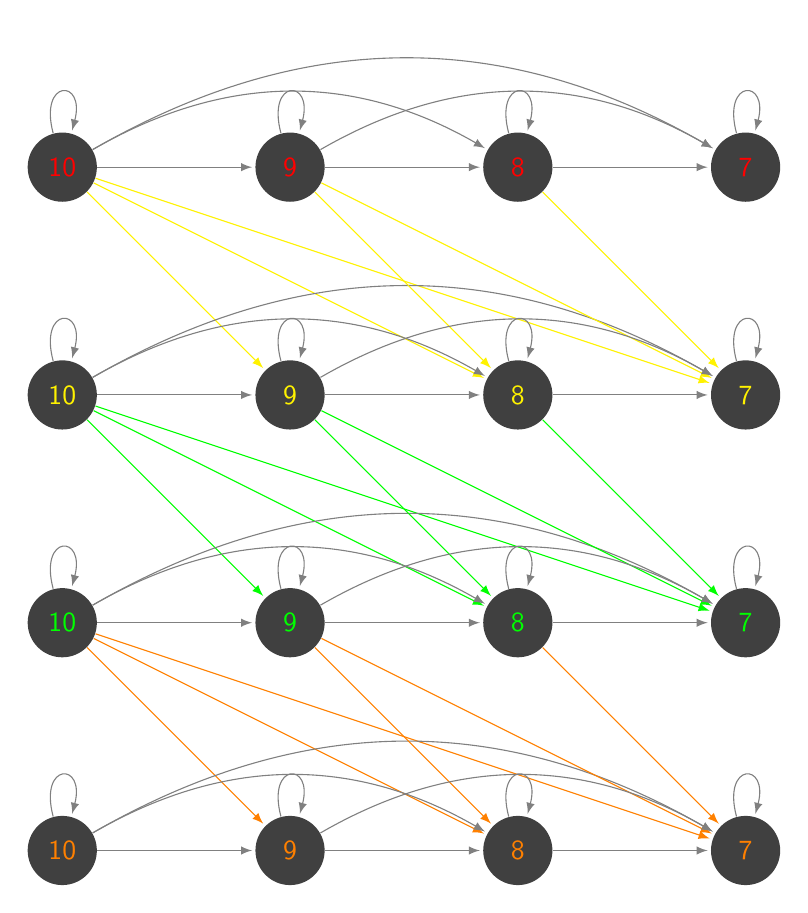
\begin{tikzpicture}[font=\sffamily]
        % Add the states
        \node[state,
              text=red,
              draw=none,
              fill=gray!50!black] (red-10) {10};
        \node[state,
              below=2cm of red-10,
              text=yellow,
              draw=none, 
              fill=gray!50!black] (orange-red-10) {10};
        \node[state,
              below=2cm of orange-red-10,
              text=green, 
              draw=none, 
              fill=gray!50!black] (green-10) {10};    
        \node[state,
              below=2cm of green-10,
              text=orange, 
              draw=none, 
              fill=gray!50!black] (orange-10) {10};                    
        \node[state,
        	  right = 2cm of red-10,
              text=red,
              draw=none,
              fill=gray!50!black] (red-9) {9};
        \node[state,
              below=2cm of red-9,
              text=yellow,
              draw=none, 
              fill=gray!50!black] (orange-red-9) {9};
        \node[state,
              below=2cm of orange-red-9,
              text=green, 
              draw=none, 
              fill=gray!50!black] (green-9) {9};    
        \node[state,
              below=2cm of green-9,
              text=orange, 
              draw=none, 
              fill=gray!50!black] (orange-9) {9};  
        \node[state,
        	  right = 2cm of red-9,
              text=red,
              draw=none,
              fill=gray!50!black] (red-8) {8};
        \node[state,
              below=2cm of red-8,
              text=yellow,
              draw=none, 
              fill=gray!50!black] (orange-red-8) {8};
        \node[state,
              below=2cm of orange-red-8,
              text=green, 
              draw=none, 
              fill=gray!50!black] (green-8) {8};    
        \node[state,
              below=2cm of green-8,
              text=orange, 
              draw=none, 
              fill=gray!50!black] (orange-8) {8};                
        \node[state,
        	  right = 2cm of red-8,
              text=red,
              draw=none,
              fill=gray!50!black] (red-7) {7};
        \node[state,
              below=2cm of red-7,
              text=yellow,
              draw=none, 
              fill=gray!50!black] (orange-red-7) {7};
        \node[state,
              below=2cm of orange-red-7,
              text=green, 
              draw=none, 
              fill=gray!50!black] (green-7) {7};    
        \node[state,
              below=2cm of green-7,
              text=orange, 
              draw=none, 
              fill=gray!50!black] (orange-7) {7};                
              
        % Connect the states with arrows
        \draw[every loop,
        auto=right,
        >=latex,
        draw=gray,
        fill=gray]
        
        	(red-10) edge[loop above](red-10)
            (red-10) edge[] (red-9)
            (red-10) edge[color = yellow](orange-red-9)
			(red-10) edge[bend left] (red-8)
			(red-10) edge[bend left] (red-7)
			(red-10) edge[color = yellow] (orange-red-8)
			(red-10) edge[color = yellow] (orange-red-7)			            
            
            (orange-red-10) edge[loop above] (orange-red-10)
            (orange-red-10) edge[] (orange-red-9)
            (orange-red-10) edge[color = green] (green-9)
            (orange-red-10) edge[bend left] (orange-red-8)
			(orange-red-10) edge[bend left] (orange-red-7)
			(orange-red-10) edge[color = green] (green-8)
			(orange-red-10) edge[color = green] (green-7)
			
        	(green-10) edge[loop above](green-10)
            (green-10) edge[] (green-9)
            (green-10) edge[color = orange](orange-9)
			(green-10) edge[bend left] (green-8)  
			(green-10) edge[bend left] (green-7)
			(green-10) edge[color = orange](orange-8)
			(green-10) edge[color = orange](orange-7)
			  
        	(orange-10) edge[loop above](orange-10)
            (orange-10) edge[] (orange-9)
			(orange-10) edge[bend left] (orange-8)  	
			(orange-10) edge[bend left] (orange-7) 

							   
							   
							         
        	(red-9) edge[loop above](red-9)
            (red-9) edge[] (red-8)
            (red-9) edge[color = yellow](orange-red-8)
			(red-9) edge[bend left] (red-7)
			(red-9) edge[color = yellow](orange-red-7)
			
	
            (orange-red-9) edge[loop above] (orange-red-9)
            (orange-red-9) edge[] (orange-red-8)
            (orange-red-9) edge[color = green] (green-8)
            (orange-red-9) edge[bend left] (orange-red-7)
            (orange-red-9) edge[color = green] (green-7)

        	(green-9) edge[loop above](green-9)
            (green-9) edge[] (green-8)
            (green-9) edge[color = orange](orange-8)
			(green-9) edge[bend left] (green-7)  
			(green-9) edge[color = orange](orange-7)
			
        	(orange-9) edge[loop above](orange-9)
            (orange-9) edge[] (orange-8)
			(orange-9) edge[bend left] (orange-7)    

			
			
        	(red-8) edge[loop above](red-8)
            (red-8) edge[] (red-7)
            (red-8) edge[color = yellow](orange-red-7)
			%(red-8) edge[bend left] (red-6)
	
            (orange-red-8) edge[loop above] (orange-red-8)
            (orange-red-8) edge[] (orange-red-7)
            (orange-red-8) edge[color = green] (green-7)
           % (orange-red-8) edge[bend left] (orange-red-6)

        	(green-8) edge[loop above](green-8)
            (green-8) edge[] (green-7)
            (green-8) edge[color = orange](orange-7)
			%(green-8) edge[bend left] (green-6)  
			
        	(orange-8) edge[loop above](orange-8)
            (orange-8) edge[] (orange-7)
			%(orange-8) edge[bend left] (orange-6) 	
			
			
			(red-7)edge[loop above](red-7)
			(orange-red-7)edge[loop above](orange-red-7)	
			(green-7)edge[loop above](green-7)	
			(orange-7)edge[loop above](orange-7)	
			
			
			
			%%%%% arrows from orange to red 
%			(orange-8) edge[color = red](red-7)	
%			(orange-9) edge[color = red](red-8)   
%			(orange-9) edge[color=red](red-7)	
%			(orange-10) edge[color = red](red-9) 	
%			(orange-10) edge[color = red](red-8)
%			(orange-10) edge[color = red](red-7)		       
            ;
    \end{tikzpicture}
    \end{center}
   \newpage
    simply a first idea : 
    \begin{itemize}
    \item the state with a number represent how far away the robot is from the traffic light (unit of distance are to be defined as explained later)
    \item the arrows represents how the robot can go from a state from another :
    \begin{enumerate}
    \item the robot can stay where he is
    \item he can either go one unit of distance or more (cf later)
    \item the traffic light can change while he is going from one distance to another : let's say it begins in $10$ with a red light and goes to $8$ if while he was arriving the traffic light changed he will go to the corresponding state \footnote{there are arrows from the orange light to the red but I didn't put them in hope it would be more readable. One can uncomment in the Latex code the arrows corresponding}
    \end{enumerate}
    \end{itemize}   

I didn't put arrows between two states 10 of different color since the change in the color of the traffic light follows an exponential distribution and hence at a precise instant the probability of changing color is 0.  1
    
    
    
    Now about the distance and velocity units, I was thinking that we could use a discretization\footnote{thanks Joachim for this idea} of the different velocities we got (I don't know maybe ten or less depends on I don't know what) and then defines a unit of our new distance as how many centimetres the robot did in one second using the lowest speed possible amongst this new set of velocities.
    
    
    
    

\end{document}